\documentclass{article}
\usepackage{pgfplots}
\pgfplotsset{compat=1.18}

\begin{document}

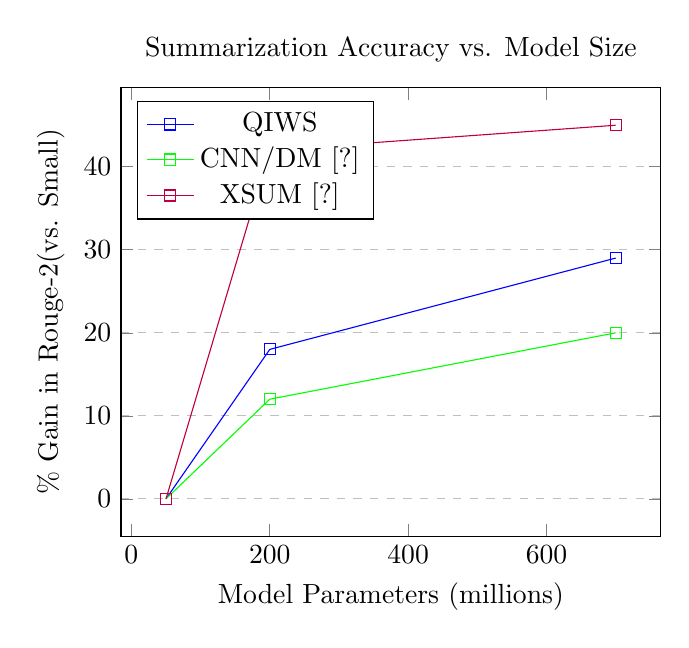
\begin{tikzpicture}
    \begin{axis}[
        title={Summarization Accuracy vs. Model Size},
        xlabel={Model Parameters (millions)},
        ylabel={\% Gain in Rouge-2(vs. Small)},
        legend pos=north west,
        ymajorgrids=true,
        grid style=dashed,
    ]
    
    % QIWS data points
    \addplot[
        color=blue,
        mark=square,
        ]
        coordinates {
            (50, 0) (200, 18) (700, 29)
        };
        \addlegendentry{QIWS}
        
    % CNN/DM data points
    \addplot[
        color=green,
        mark=square,
        ]
        coordinates {
            (50, 0) (200, 12) (700, 20)
        };
        \addlegendentry{CNN/DM [?]}
        
    % XSUM data points
    \addplot[
        color=purple,
        mark=square,
        ]
        coordinates {
            (50, 0) (200, 42) (700, 45)
        };
        \addlegendentry{XSUM [?]}
        
    \end{axis}
\end{tikzpicture}

\end{document}